\begin{frame}[label=title]
    \centering
    \begin{figure}[H]
        
\includegraphics[keepaspectratio, width=0.7\paperwidth, height=\paperheight]{LeeLogo}
    \end{figure}
    Informatik: Data Science und Sicherheit\\
    \textbf{Lektion 5} \emoji{chart-increasing}: \textbf{Kryptoanalyse}
\end{frame}


\begin{frame}[label=repetition]{Geheimschriften: \emoji{cat}- und \emoji{mouse}-Rennen}
	\begin{multicols}{2}
		\textbf{Kryptologie}
		\begin{itemize}
			\item Geheimschrift mit vertauschten Buchstaben
			\item Skytale
			\item Caesar
		\end{itemize}
		\columnbreak
		\textbf{Kryptoanalyse}
		\begin{itemize}
			\item Geheimschriften analysieren
			\item 25 Verschiebungen ausprobieren
			\item Statistische Analyse
		\end{itemize}
	\end{multicols}
\end{frame}

\begin{frame}[label=repetition2]
	{Wiederholung letztes Mal}
	\begin{figure}[H]
		\centering
		\raisebox{-0.5\height}{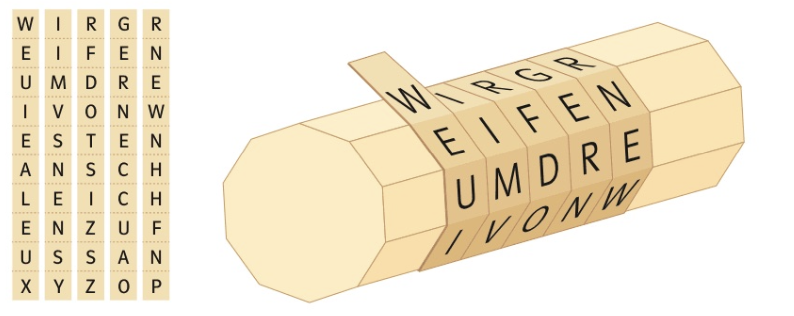
\includegraphics[width=.35\linewidth]{GrundlagenInfo/DataScience/03_Kryptologie/Figures/skytale.png}}
		\raisebox{-0.5\height}{$\rightarrow$ Tabellengrössen ausprobieren}
		\raisebox{-0.5\height}{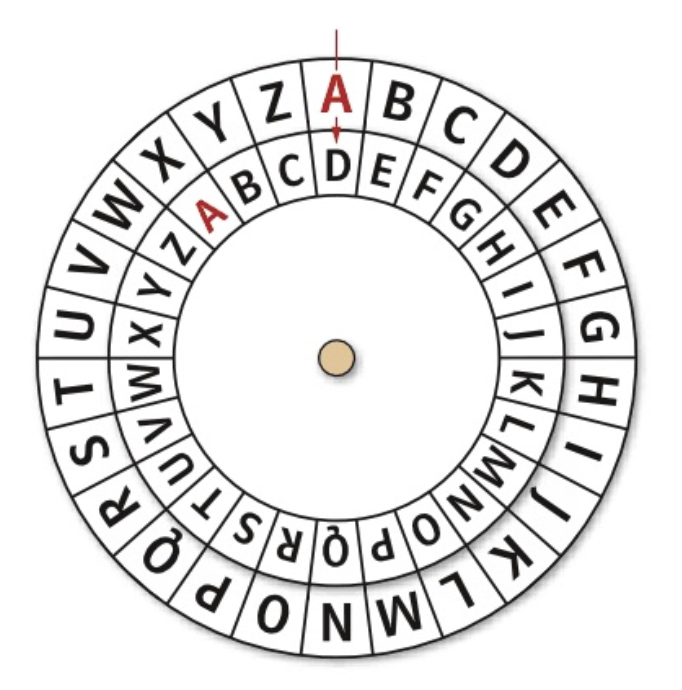
\includegraphics[width=.35\linewidth]{GrundlagenInfo/DataScience/03_Kryptologie/Figures/caesar.png}}
		\raisebox{-0.5\height}{$\rightarrow$ 25 Verschiebungen ausprobieren}
		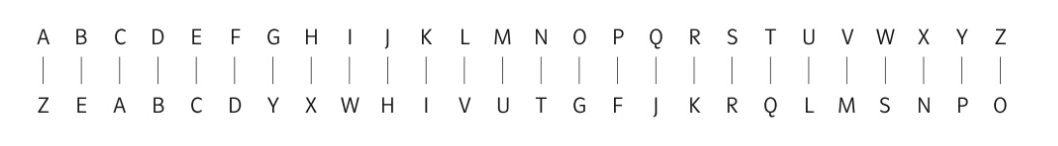
\includegraphics[width=\linewidth]{GrundlagenInfo/DataScience/03_Kryptologie/Figures/multikey.png}
		$\rightarrow$ \textbf{Wie knacken wir so etwas?}
	\end{figure}

\end{frame}

\begin{frame}[fragile, label=hauefigkeit]{Häufigkeitsverteilung}
	\begin{multicols}{2}
		    \begin{figure}[H]
			\centering
			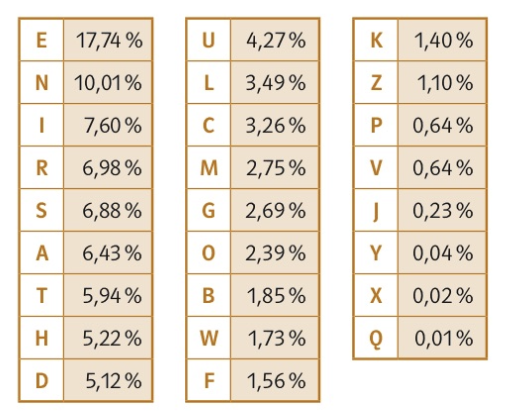
\includegraphics[width=\linewidth]{GrundlagenInfo/DataScience/03_Kryptologie/Figures/freq.png}
		\end{figure}
		\columnbreak
		\[h_\square (T)\]
		= Häufigkeit von Buchstabe $\square$ in Text $T$.
	\end{multicols}
    \begin{figure}[H]
    	\centering
    	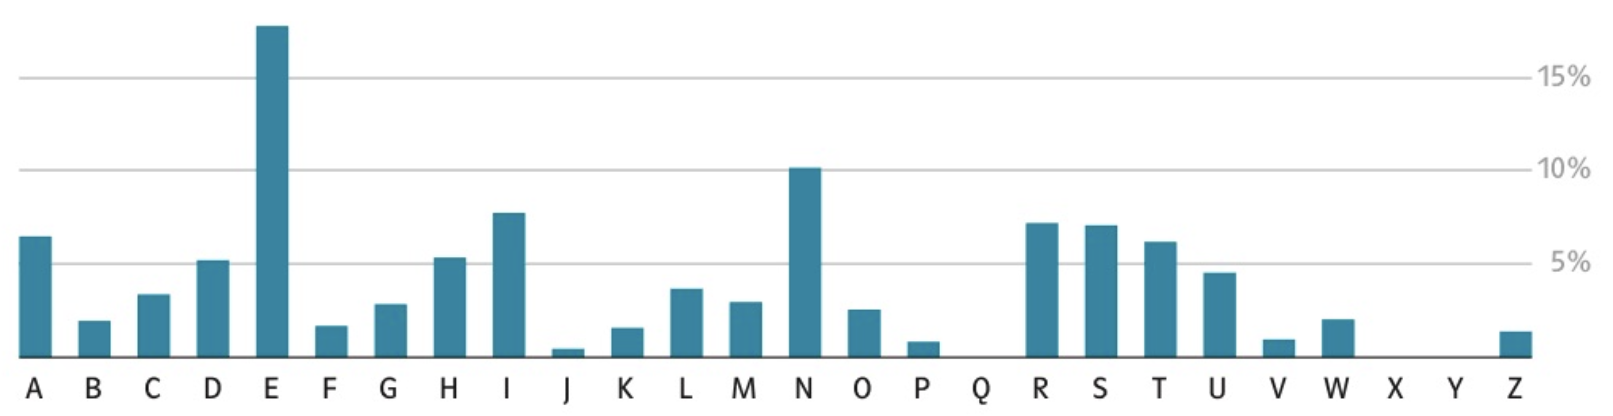
\includegraphics[width=\textwidth]{GrundlagenInfo/DataScience/03_Kryptologie/Figures/friedmann1-klartext.png}
    \end{figure}
\end{frame}

\begin{frame}[fragile]{Häufigkeitsanalyse}
    $h_\square (T)$ im deutschen Alphabet:
	\begin{figure}[H]
	        \centering
	        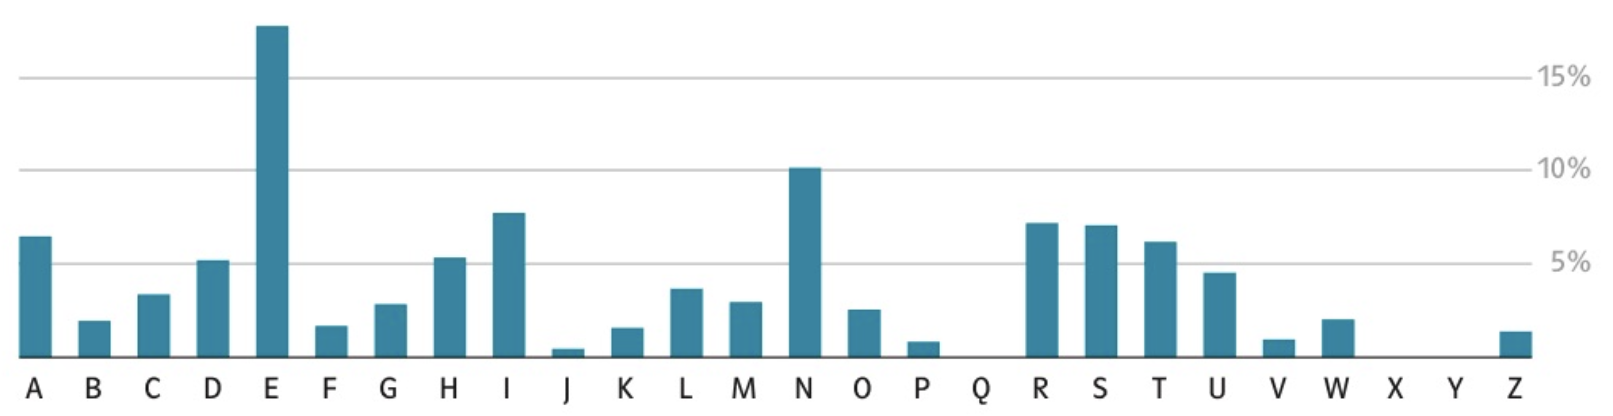
\includegraphics[width=\textwidth]{GrundlagenInfo/DataScience/03_Kryptologie/Figures/friedmann1-klartext.png}
	\end{figure}
	$h_\square (T)$ in einem monoalphabetisch verschlüsselten Text:
	\begin{figure}[H]
	        \centering
	        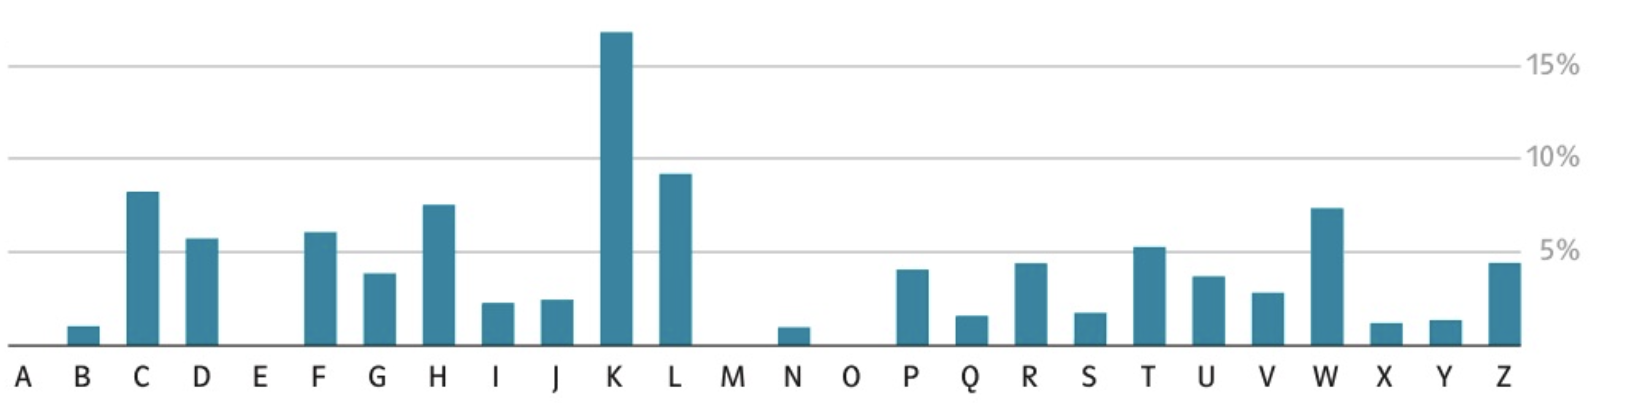
\includegraphics[width=\textwidth]{GrundlagenInfo/DataScience/03_Kryptologie/Figures/friedmann1-geheimtext.png}
	\end{figure}
\end{frame}


\begin{frame}[fragile]{Häufigkeitsanalyse}
\textbf{Problem}: Alle \textbf{monoalphabetischen} Kryptosysteme lassen sich mit einfacher Häufigkeitsanalyse knacken
    \begin{figure}[H]
        \centering
        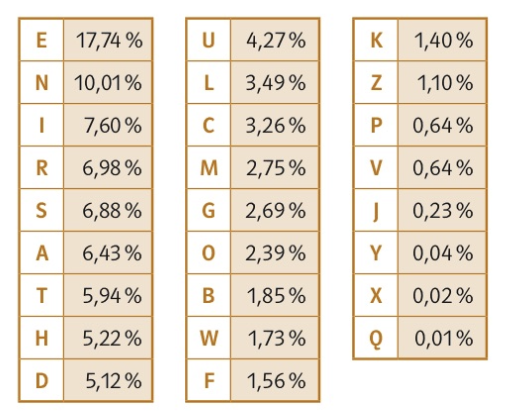
\includegraphics[width=.55\linewidth]{GrundlagenInfo/DataScience/03_Kryptologie/Figures/freq.png}
        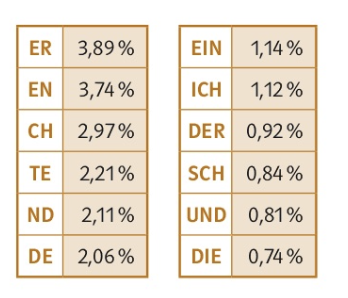
\includegraphics[width=.4\linewidth]{GrundlagenInfo/DataScience/03_Kryptologie/Figures/bigramme.png}
    \end{figure}
    \textcolor{red}{\rule{\textwidth}{.3mm}}\\[-.1cm]
    \defverbatim{\verbOne}{
    \small\begin{verbatim}
MUMMUXJUQYMHQOUSUTUQNGWTJQVHUMXQUXQJSUVYPPUM
--------------------------------------------
    \end{verbatim}
    U kommt 10-mal vor, M kommt 6-mal vor, Q kommt 6-mal vor
    }
    
    \defverbatim{\verbTwo}{
    \small\begin{verbatim}
MUMMUXJUQYMHQOUSUTUQNGWTJQVHUMXQUXQJSUVYPPUM
NENNE--EI-N-I-E-E-EI-----I--EN-IE-I--E----EN
    \end{verbatim}
    U=E, M=N, Q=I?
    }
    
    \defverbatim{\verbThree}{
    \small\begin{verbatim}
MUMMUXJUQYMHQOUSUTUQNGWTJQVHUMXQUXQJSUVYPPUM
NENNED-EI-N-I-E-E-EI-----I--ENDIEDI--E----EN
\end{verbatim}
Wir fahren nun mit Trigrammen weiter: ``Die''?
    }

    \defverbatim{\verbFour}{
    \small\begin{verbatim}
MUMMUXJUQYMHQOUSUTUQNGWTJQVHUMXQUXQJSUVYPPUM
NENNEDREI-N-I-E-E-EI----RI--ENDIEDIR-E----EN
\end{verbatim}
``D-EI''=``Drei''?
    }

    \defverbatim{\verbFive}{
    \small\begin{verbatim}
MUMMU|XJUQ|YMHQOUSUTUQNGWTJQVHUM|XQU|XQJ|SUVYPPUM
NENNE|DREI|-N-I-E-E-EI----RI--EN|DIE|DIR|-E----EN
\end{verbatim}
Man beginnt Wörter zu erkennen
    }

    \defverbatim{\verbSix}{
    \small\begin{verbatim}
MUMMU|XJUQ|YMHQOU|SUTUQNGWTJQVHUM|XQU|XQJ|SUVYPPUM
NENNE|DREI|ANTIKE|GEHEIMSCHRIFTEN|DIE|DIR|GEFALLEN
    \end{verbatim}
    \emoji{blush}
    }
    
    \only<1>{\verbOne}
    \only<2>{\verbTwo}
    \only<3>{\verbThree}
    \only<4>{\verbFour}
    \only<5>{\verbFive}
    \only<6>{\verbSix}
\end{frame}

\begin{frame}{Mono- und Polyalphabetische Kryptosysteme}
	\begin{itemize}[<+->]
		\item \textbf{Monoalphabetisch}: Jeder Buchstabe wird immer durch denselben Buchstaben erstetzt, unabhängig von seiner Position im Klartext
		\begin{figure}[H]
			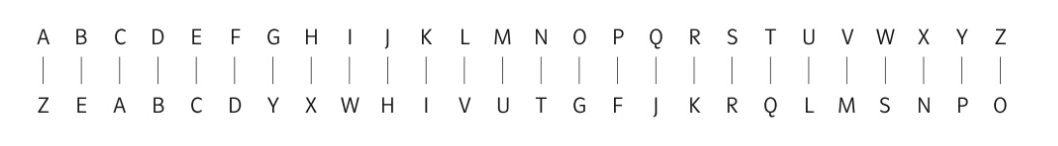
\includegraphics[width=\linewidth]{GrundlagenInfo/DataScience/03_Kryptologie/Figures/multikey.png}
		\end{figure}
		Nachteil: Einfache Entschlüsselung durch Häufigkeitsanalyse
		\item \textbf{Polyalphabetisch}: Jeder Buchstabe kann durch unterschiedliche Buchstaben ersetzt werden
	\end{itemize}
\end{frame}

\begin{frame}{Kerkhoffs'sches Prinzip der Sicherheit}
	\begin{center}
		``Ein Kryptosystem ist \textbf{sicher}, wenn das Kryptosystem [= der Algorithmus] öffentlich bekannt ist und es trotzdem ohne die Kenntnis des verwendeten Schlüssels nicht möglich ist, aus einem Geheimtext den ursprünglichen Klartext abzuleiten.''
	\end{center}    
\end{frame}

\begin{frame}[label=jv]{Jules Verne \emoji{scroll}}
	\begin{figure}[H]
	        \centering
	        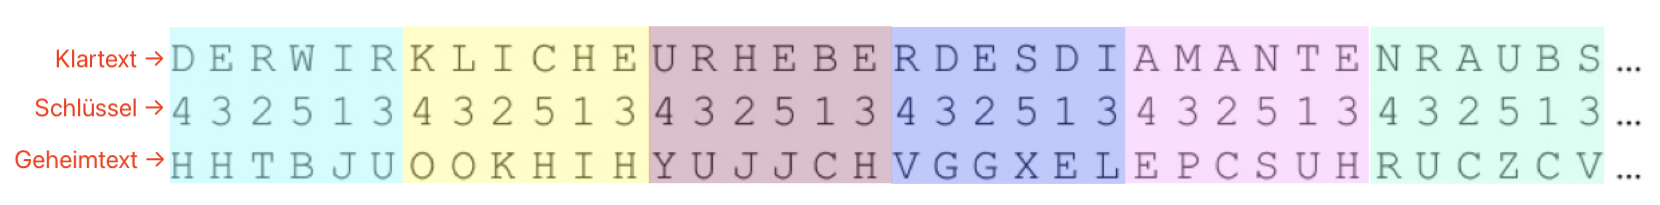
\includegraphics[width=\linewidth]{GrundlagenInfo/DataScience/03_Kryptologie/Figures/julesverne2.png}
	\end{figure}
	\begin{itemize}[<+->]
	    \item \emoji{check-mark-button} Vorteil: nicht mehr monoalphabetische, sondern polyalphabetische Verschlüsselung
	    \item \emoji{check-mark-button} Ein ``E'' kann nun beispielsweise um 1 (F), 2 (G), 3 (H), 4 (I) oder 5 (J) Positionen verschoben sein.
	    \item \emoji{thinking-face} Problem: Nur 9 Schlüssel, einfach zu knacken bei bekannter Schlüssellänge...
	\end{itemize}
\end{frame}

\begin{frame}[label=vigenere]{Vigenère \emoji{fleur-de-lis}}
\begin{figure}[H]
        \centering
        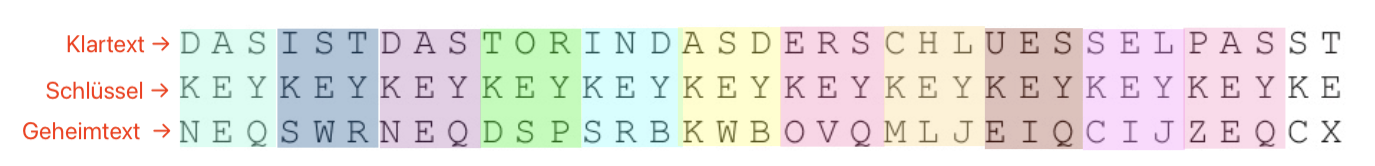
\includegraphics[width=\linewidth]{GrundlagenInfo/DataScience/03_Kryptologie/Figures/vigenere1.png}
\end{figure}
\begin{itemize}[<+->]
	\item Verallgemeinerung von Jules Verne
    \item B=Verschiebung um 1 Position, C=Verschiebung um 2 Positionen, usw.
    \item Allgemein: Verschiebung = $\text{Ord}(\square)$, wobei $\text{Ord}(A)=0$
    \item 25 mögliche Schlüssel
    \item nicht \textbf{monoalphabetisch} sondern \textbf{polyalphabetisch}
    \item Galt über 300 Jahre lang als sicher!
\end{itemize}
\end{frame}

\begin{frame}[label=vigenere2]{Vigenère \emoji{fleur-de-lis}}
\begin{figure}[H]
	        \centering
	        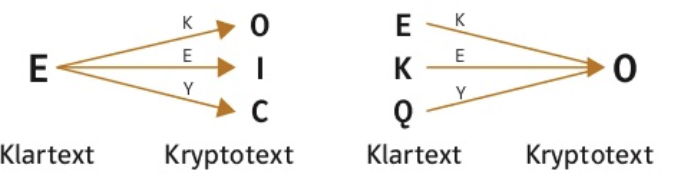
\includegraphics[width=.6\linewidth]{GrundlagenInfo/DataScience/03_Kryptologie/Figures/vigenere2.png}
	\end{figure}
	\begin{align*}
	    h_{Geheimtext}(O) &= \frac{h_{Klartext}(E)+h_{Klartext}(K)+h_{Klartext}(Q)}{3} \\
	    &= \frac{17.7\%+1.4\%+0.01\%}{3}=6.4\%
	\end{align*}
	$\rightarrow$ Die Häufigkeiten der Buchstaben entsprechen nun nicht mehr direkt einer Häufigkeit eines anderen Buchstabens im Originaltext!
\end{frame}
\begin{frame}[label=kasiskiKeyFixed]{Angriff auf Vigenère: Bekannte Schlüssellänge}
	\textbf{Beispiel}: Geheimtext mit Schlüssellänge 3
	\only<1>{
	\begin{figure}[H]
	        \centering
	        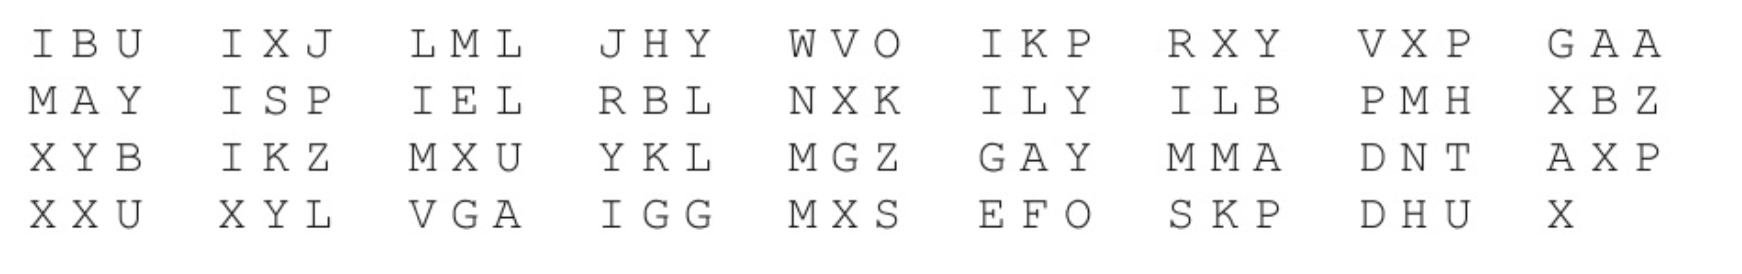
\includegraphics[width=\linewidth]{GrundlagenInfo/DataScience/03_Kryptologie/Figures/vigenereKeyFixed1.png}
	\end{figure}
	}
	
	\only<2->{
	\begin{figure}[H]
	        \centering
	        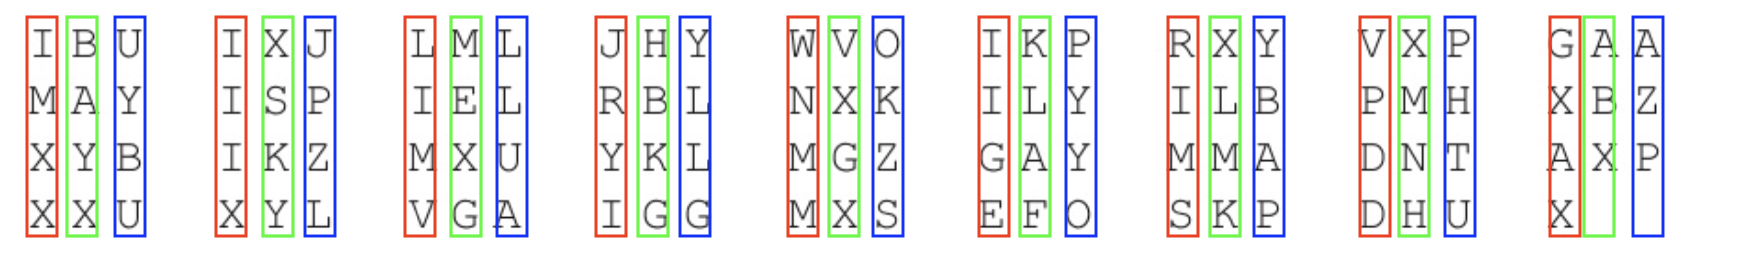
\includegraphics[width=\linewidth]{GrundlagenInfo/DataScience/03_Kryptologie/Figures/vigenereKeyFixed2.png}
	\end{figure}
	}
	\only<3>{\textbf{Häufigkeitsanalyse} pro Gruppe (rot, grün, blau):\\
	\begin{figure}[H]
	        \centering
	        \raisebox{-0.5\height}{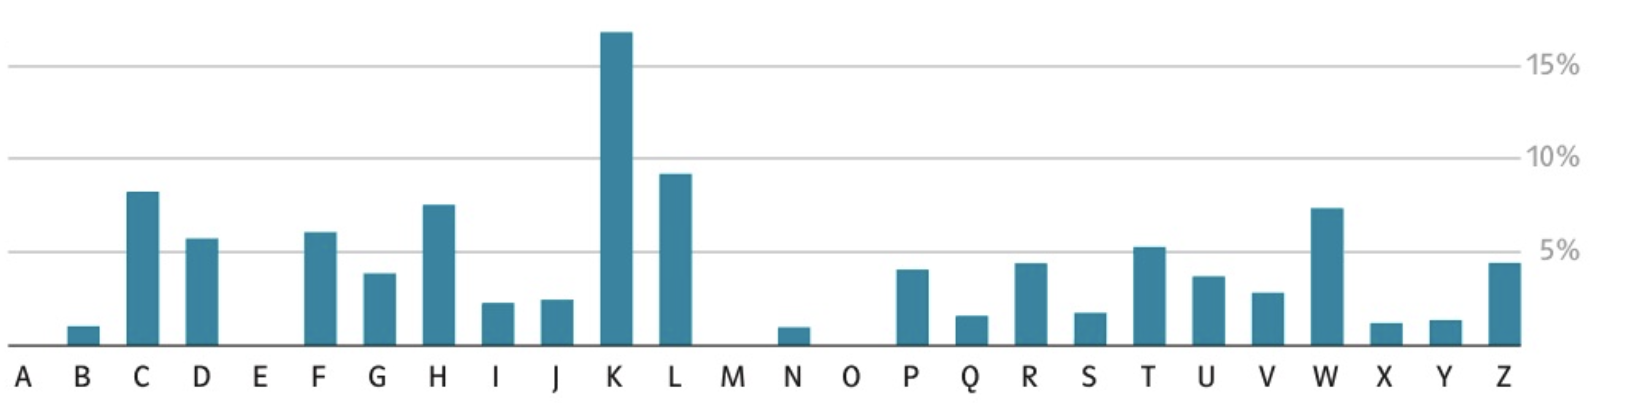
\includegraphics[width=.45\textwidth]{GrundlagenInfo/DataScience/03_Kryptologie/Figures/friedmann1-geheimtext.png}}
	        \raisebox{-0.5\height}{$\rightarrow$}
	        \raisebox{-0.5\height}{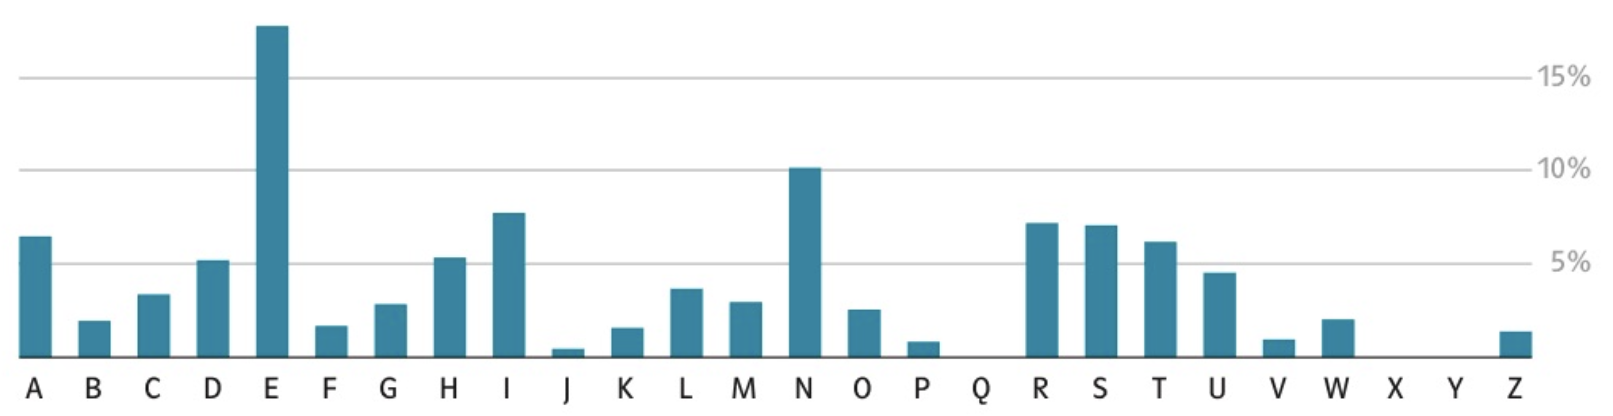
\includegraphics[width=.45\textwidth]{GrundlagenInfo/DataScience/03_Kryptologie/Figures/friedmann1-klartext.png}}
	\end{figure}}
\end{frame}



\begin{frame}[label=kasiski]{Angriff auf Vigenère: Unbekannte Schlüssellänge}{\textbf{Kasiski-Test}}
\emoji{key} Schlüssellänge unbekannt!\\[1cm]
\texttt{DER KLAR\textbf{TEXT} WERDE GEHEIM\textbf{TEXT}\\
PLU TOPL\textbf{UTOP} LUTOP LUTOPL\textbf{UTOP}\\
SPL DZPC\textbf{NXLI} HYKRT RYASXX\textbf{NXLI}}\\[1cm]

\begin{itemize}
    \item ``\texttt{NXLI}'' kommt zweimal im Geheimtext vor
    \item Distanz zwischen \texttt{NXLI} = Vielfaches der Schlüssellänge
\end{itemize}
\end{frame}
\begin{frame}[label=kasiski2]{Angriff auf Vigenère: \textbf{Kasiski-Test}}
\only<1>{
Angenommen, wir haben folgenden Text, verschlüsselt mit dem Wort ``BALMER'':
\begin{figure}[H]
        \centering
        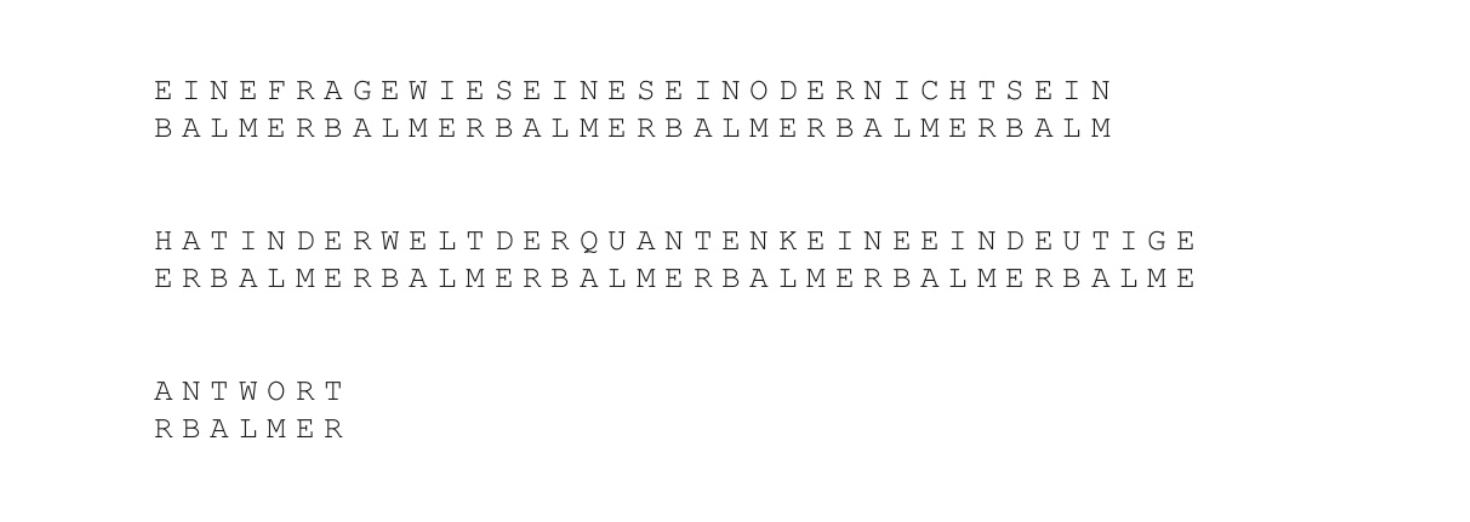
\includegraphics[width=\textwidth]{GrundlagenInfo/DataScience/03_Kryptologie/Figures/Kasiski1.png}
\end{figure}
}
\only<2>{
Wir suchen nun zuerst im Geheimtext nach Trigrammen, die mehrmals vorkommen:
\begin{figure}[H]
        \centering
        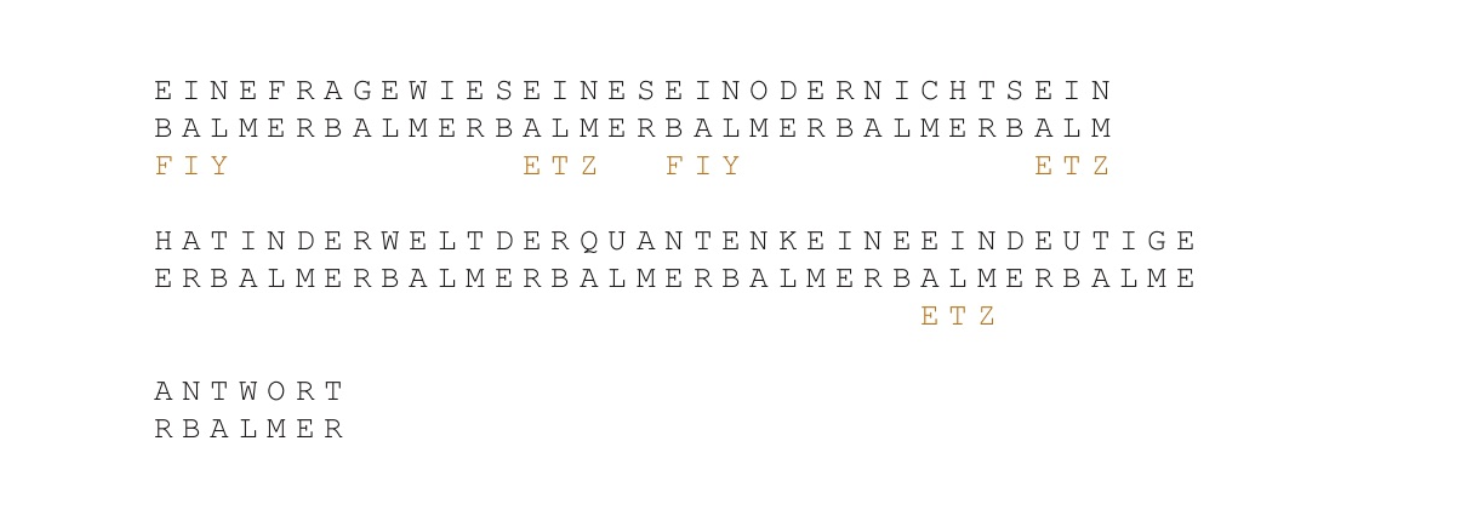
\includegraphics[width=\textwidth]{GrundlagenInfo/DataScience/03_Kryptologie/Figures/Kasiski2.png}
\end{figure}
}
\only<3>{
Wir notieren die Anfangs-Positionen der Trigramme:
\begin{figure}[H]
        \centering
        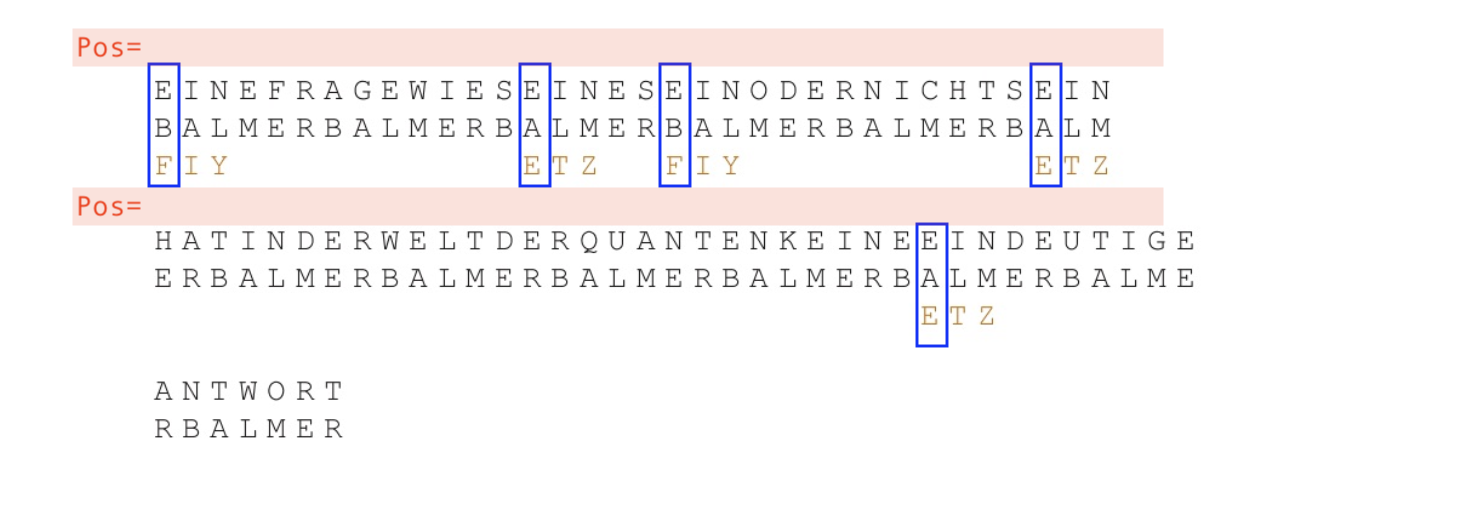
\includegraphics[width=\textwidth]{GrundlagenInfo/DataScience/03_Kryptologie/Figures/Kasiski3.png}
\end{figure}
}
\only<4->{
Wir notieren die Anfangs-Positionen der Trigramme:
\begin{figure}[H]
        \centering
        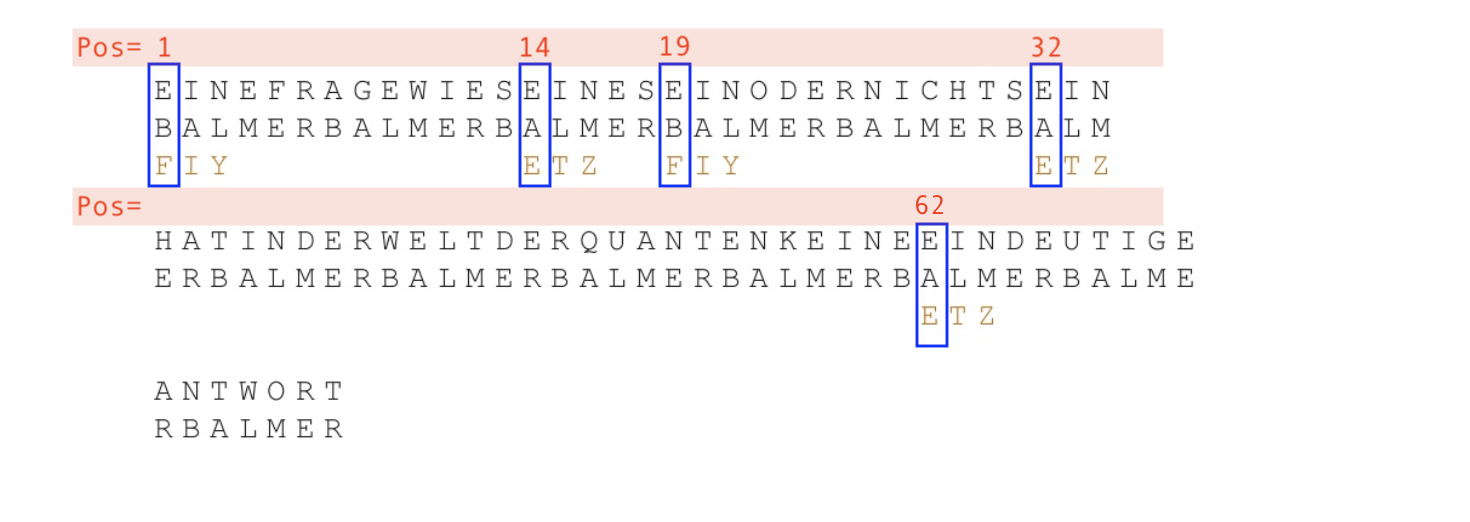
\includegraphics[width=\textwidth]{GrundlagenInfo/DataScience/03_Kryptologie/Figures/Kasiski4.png}
\end{figure}
}
\only<5->{
Nun können wir die Abstände zwischen den mehrfach vorkommenden Trigrammen berechnen:
\begin{align*}
62 - 14 = 48 = 2^4\cdot 3\\
62 - 32 = 30 = 2 \cdot 3 \cdot 5\\
32 - 14 = 18 = 2 \cdot 3^2
\end{align*}
GGT = 6 $\rightarrow$ Länge des Schlüsselworts.
}
\end{frame}



\begin{frame}[fragile,label=friedmann]{Friedmann'sche Charakteristik}
\only<1>{
$h_\square (T)$ im deutschen Alphabet:
\begin{figure}[H]
        \centering
        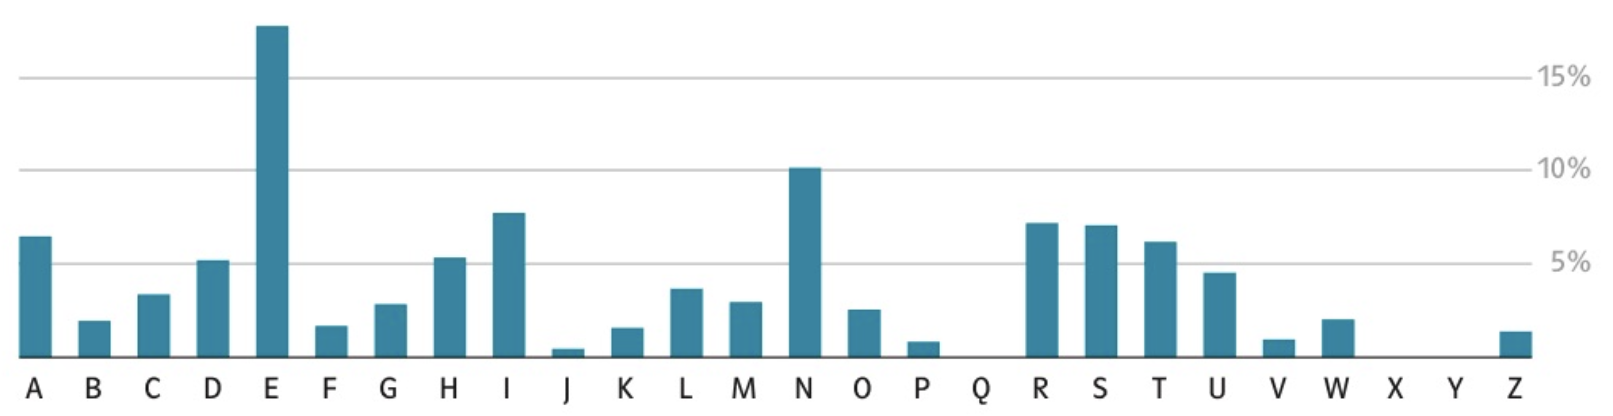
\includegraphics[width=\textwidth]{GrundlagenInfo/DataScience/03_Kryptologie/Figures/friedmann1-klartext.png}
\end{figure}
$h_\square (T)$ in einem monoalphabetisch verschlüsselten Text:
\begin{figure}[H]
        \centering
        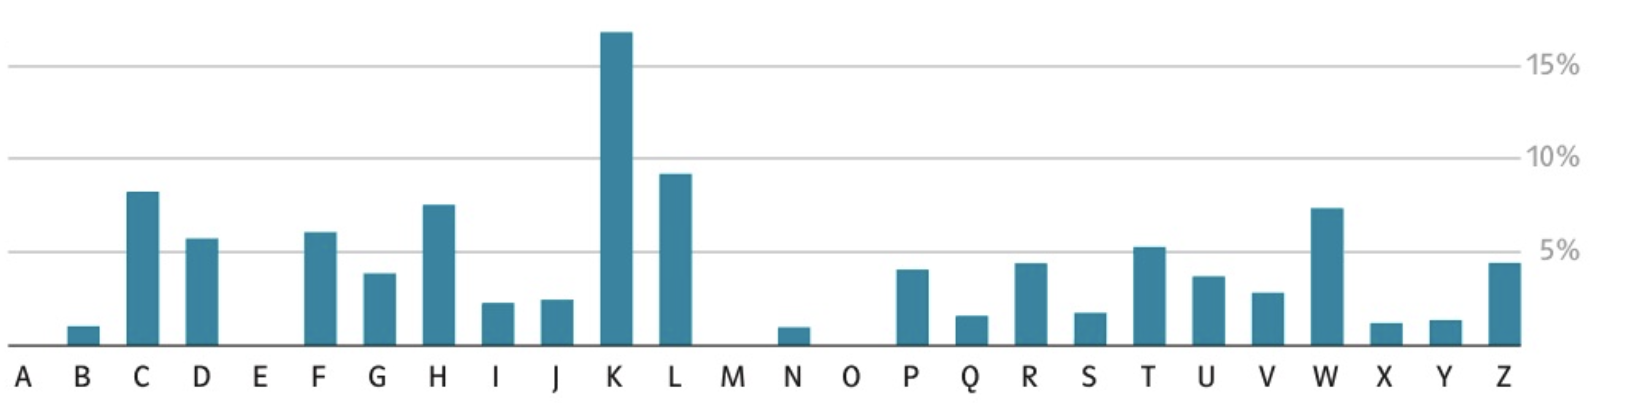
\includegraphics[width=\textwidth]{GrundlagenInfo/DataScience/03_Kryptologie/Figures/friedmann1-geheimtext.png}
\end{figure}
}
\only<2-3>{
Durchschnittliche Abweichung vom Mittelwert:
\begin{figure}[H]
        \centering
        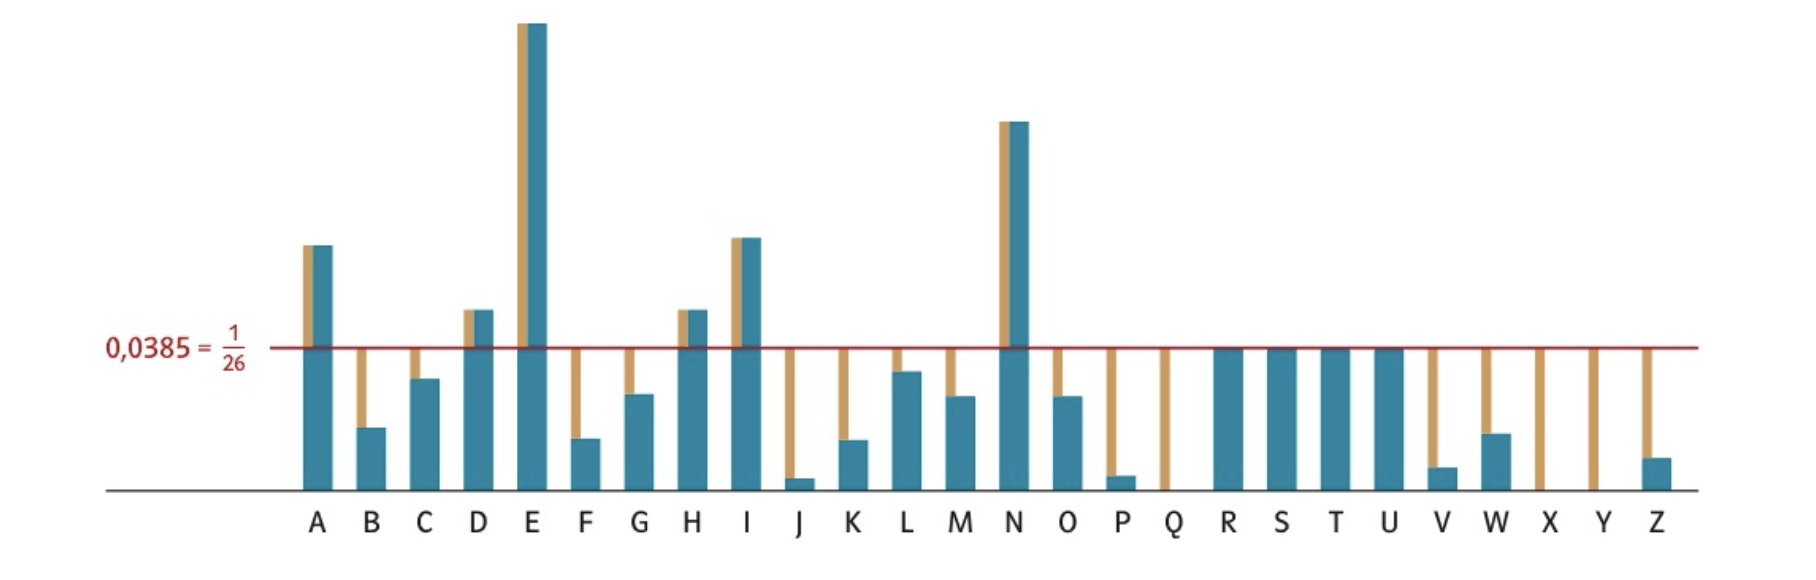
\includegraphics[width=\textwidth]{GrundlagenInfo/DataScience/03_Kryptologie/Figures/friedmann2.png}
\end{figure}

}
\only<3>{
\begin{align*}
    FC(T)&=\big(h_A(T)-\frac{1}{26}\big)^2+\big(h_B(T)-\frac{1}{26}\big)^2+\ldots+\big(h_Z(T)-\frac{1}{26}\big)^2\\
    &=\sum_{\Delta\in \text{Alphabet}}\big(h_\Delta(T)-\frac{1}{26}\big)^2
\end{align*}
\emoji{flag-germany} $FC(T)\sim 0.0388$ für deutsche Texte 
}

\only<4>{
\textit{Brute force}-Ansatz, um Wortlänge von Vigenère zu berechnen: 
\begin{enumerate}
    \item Alle möglichen Wortlängen von 1 bis $n$ ausprobieren
    \item Buchstaben jeweils in Gruppen unterteilen
    \item Durchschnittliche $FC(T)$ für alle Gruppen berechnen. 
    \item Wenn die richtige Länge gewählt wurde, sollte $FC(T)\sim 0.0388$ sein. Falls nicht, mit nächstgrösserer Wortlänge weitermachen.
\end{enumerate}
    
\begin{figure}[H]
        \centering
        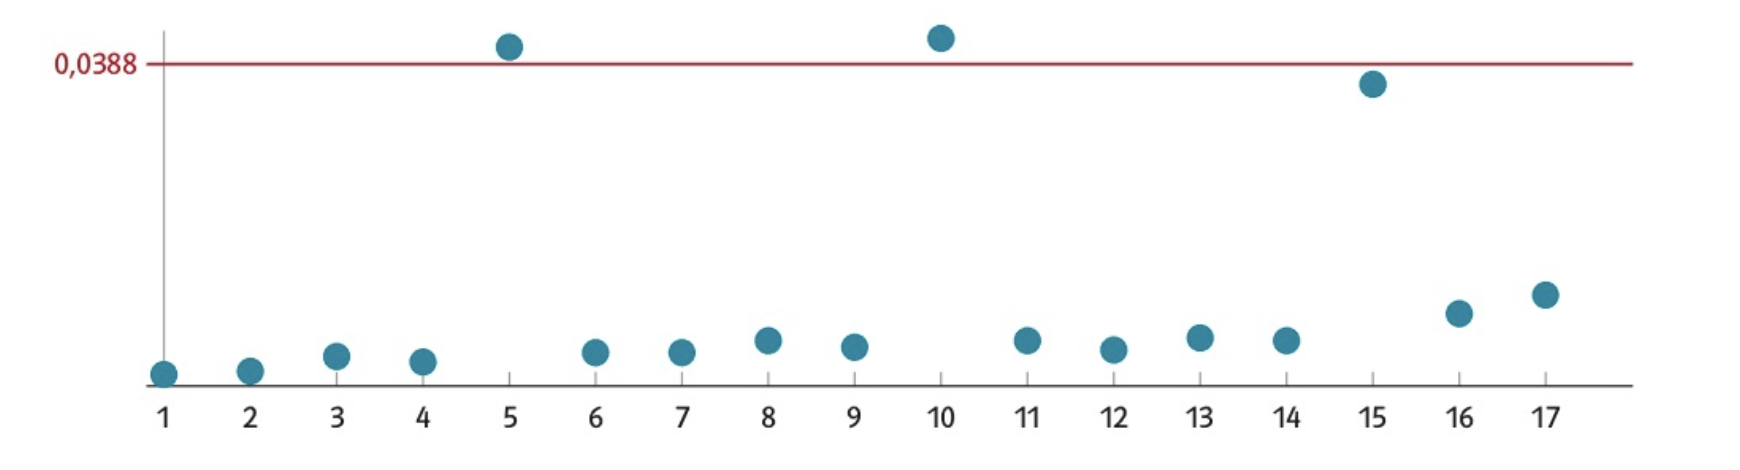
\includegraphics[width=\textwidth]{GrundlagenInfo/DataScience/03_Kryptologie/Figures/friedmann3.png}
\end{figure}
$\rightarrow$ Hier sehen wir visuell, dass die Wortlänge 5 sein muss.
}
\end{frame}

\begin{frame}[label=auftrag]{Auftrag}
	\begin{itemize}
		\item Kopieren Sie den Geheimtext (Vigenère) von Moodle und versuchen Sie, ihn mit dem Analysetool zu entziffern
		\item \emoji{trophy} Challenge: Versuchen Sie, die Challenge-Aufgabe auf Moodle zu lösen
	\end{itemize}
\end{frame}


\begin{frame}[label=auftrag]{\emoji{trophy} Challenge-Auftrag}
	\small
Teil 1: Verschlüsselung
\begin{itemize}
	\item Erstellen Sie einen Text in deutscher Sprache mit mindestens 1000 Zeichen, beispielsweise mittels folgender Webseite: \url{https://www.blindtextgenerator.de/}
	\item Wählen Sie ein \textit{geheimes} Schlüsselwort (3-7 Zeichen) und verschlüsseln Sie die Nachricht mit Vigenère (s. Moodle, Python-Datei 1).
\end{itemize}
Teil 2: Entschlüsselung
\begin{itemize}
	\item Zuerst wird die Schlüssellänge per Friedmann-Test bestimmt  (s. Moodle, Python-Datei 2). 
	\item Danach wird innerhalb jeder Gruppe der häufigste Buchstabe gesucht. Dieser entspricht mit hoher Wahrscheinlichkeit dem Buchstaben ``E'', somit haben wir die Verschiebung für diese Wort-Gruppe gefunden und damit auch das Schlüsselwort  (s. Moodle, Python-Datei 3).
	\item Der Text kann nun wieder mit dem Vigenère-Programm entschlüsselt werden  (s. Python-Datei 1). 
\end{itemize}
\normalsize
\end{frame}

%\begin{frame}[label=auftrag]{Auftrag}
%\begin{itemize}
%    \item Aufgabe 2.27 (Häufigkeitsanalyse)
%    \item Aufgabe 2.28 (Monoalphabetische Verschlüsselung)
%    \item Aufgabe 2.35 (Vigenère)
%    \item Aufgabe 2.40 (Kasiski-Test)
%    \item Aufgabe 2.42 (Friedmann'sche Charakteristik)
%\end{itemize}
%\end{frame}
